\subsection{}
First let us extend the alphabet $\Sigma$ to $\Sigma' = \Sigma \cup \{\epsilon\}$ where $\epsilon$ is the empty sting. Now for each state $s\in S$, $e_s(\epsilon) = 1 - \sum_{a\in \Sigma} e_s(a)$ hence $\sum_{a\in \Sigma'} e_s(a) = 1$. Using epsilon we can now consider the problem as finding the most likely sequence of states to generate our sequence, $O$, of $n$ letters with any amount of $\epsilon$ in $O$ at any position.

The Viterbi Algorithm can be described mathmatically as:
\begin{align*}
\textbf{Base Case: } &\delta_1(i) = \pi_i e_i(O_1)\\
\textbf{Inductive Case: } &\delta_t(j) = \max_{1\leq i \leq N}[\delta_{t-1}(i)m_{ij}]\cdot e_j(O_t)
\end{align*}

Our new algorithm will extend the Viterbi algorithm. As a high level explanation, our new algorithm will no longer assume that in the inductive step that we directly transition from state $i$ to $j$ with probability $m_{ij}$. Instead it will allow any path from $i$ to $j$ where any intermediate states will emit $\epsilon$. Given we are findingg a maxium probability we need only consider the most likely path from $i$ to $j$. To describe this path we will define $\psi(i,j)$ as the maximum path from $i$ to $j$ where transitions $x$ to $y$ must emit $\epsilon$ unless $x=i$ (as we know $i$ has already emmited letter $O_t$).

You can calculate $\psi$ using Dijksta's algorithm. To do this we will use Dijkstra's to find the maximal path from a specified starting state $i$ to all other states. This will complete entries $\psi(i,j)  \forall j \in S:j\neq i$. Doing this for each state $i$ will mostly complete $\psi$. To fully complete $\psi$, we just need to fill in all $\psi(i,i)$ which is just $m_{ii}$.
The graph we preform Djikstas on has a vertex for each state in $S$. The graph is fully connected. Edge weights are $m_{xy}\cdot e_x(\epsilon)$ for each node $x$ except when $x=i$ then the edge weights are $m_iy$. It is not imedietly apparent how you can preform Djikstas to maximise a product of probabilities however there are 2 options. You could transform every proability into a negative log proability, then minimise the sum of negative log probabilities; You can run the sstandard definition of Dijksta's on this graph. Or you can slightly modiy Dijksta so where we use minimum distances we now use maximum distances; and where wwe calculate the sum of distances we instead take the product.

Defining $\psi$ is the first step, the next we need to consider the base case for Viterbi. As is, the Viterbi algorithm assumes we instantly emmit the first state, however this is not the case now we can emit $\epsilon$ as we may have empty strings at the begining before $O_1$. the solution to this is to define a new function $\Pi$. Much like $\psi$, $\Pi(i)$ will be the most probable path from the starting state to $i$. We can calculate this again using Dijkstra's using a graph where we have 1 vertex for every state and an extra start vertex. Edges between 2 states $i,j$ have weight $m_{ij}*e_i{\epsilon}$. Edges from the start vertex to states $i$ have wight $\pi_i$.

Using the tools we have created we can now adapt the Viterbi Algorithm to solve the problem.


\begin{align*}
    \textbf{Base Case: } &\delta_1(i) = \Pi_i e_i(O_1)\\
    \textbf{Inductive Case: } &\delta_t(j) = \max_{1\leq i \leq N}[\delta_{t-1}(i)\psi(i,j)]\cdot e_j(O_t)
    \end{align*}
\subsection{}
A hidden markov model can be defined as $\lambda = (\pi, m, e)$ where: $\pi$ are the initial probabilities, $m$ are the transition probabilities, and $e$ are the emission probabilities.
The goal of the Expectation Maximisation algorithm is to calculate a value of $\lambda$ that maximises $p(x|\lambda)$ for a given sequence of observed data $x$. As finding a global maximum is computationally intractable we use the Baum-Welch algorithm which gives us a local maximum. The Baum-Welch algorithm generates $\hat{\lambda}$ from $\lambda$ where $p(x|\hat{\lambda}) \geq p(x|\lambda)$. Iterating this process, where at each step we say $\lambda \gets \hat{\lambda}$, converges to a local optimum.

To calculate $\hat{\lambda}$ we can use some helper functions as described by L.R. Rabiner \cite{em}. We will use additional notation $N$ ass the number of hidden states, $O_t$ the observation at time (position) $t$ and $T$ as $|O|$.  The first helper function is $\alpha$, which is the forward algorithm.
\begin{gather*}
    \alpha_1(i) = \pi_i e_i(O_1)\\
    \alpha_{t+1}(i) = e_j(O_{t+1}) \cdot \sum_{i=1}^N\alpha_t(i)m_{ij}
\end{gather*}

The next $\beta$, which is the backward algorithm :
\begin{gather*}
    \beta_T(i)=1\\
    \beta_t(i)=\sum_{j=1}^N m_{ij} e_j(O_{t+1}) \beta_{t+1}(j)
\end{gather*}

Then $\gamma$ which is the probability of being in a state at a point in time, given we know which observations precede and succeed the current observation.
\begin{gather*}
    \gamma_t(i) = \frac{\alpha_t(i) \beta_t(i)}{\sum_{j=1}^N \alpha_t(j) \beta_t(j)}
\end{gather*}

And finally $\xi$, the probability of transitioning from state i to state j given we know all observations preceding i and succeeding j.
\begin{gather*}
    \xi_t(i, j) = \frac{\alpha_t(i) m_{ij} e_j(O_{t+1}) \beta_{t+1}(j)}{\sum_{i=1}^N \sum_{j=1}^N \alpha_t(i) m_{ij} e_j(O_{t+1}) \beta_{t+1}(j)}
\end{gather*}

Using these helper functions we can calculate $\hat{\lambda}=(\hat{\pi}, \hat{m}, \hat{e})$.
\begin{gather*}
    \hat{\pi}_i = \gamma_1(i)\biggbreak
    \hat{m}_{ij} = \frac{\sum_{t=1}^{T-1} \xi_t(i,j)}{\sum_{t=1}^{T-1} \gamma_t(i)}\biggbreak
    \hat{e}_i(k) \frac{\sum_{\forall t: O_t = k} \gamma_t(i)}{\sum_{t=1}^T \gamma_t(i)}
\end{gather*}


We can tackle verification of the algorithm using 2 methods: by testing helper function and by observing that the algorithm maximises $p(x|\lambda)$. I verified each helper function with unit tests that: verify base cases (if applicable); and verify against known mathematical identities. Following are a small sample of the 8 identities I test against. NOTE: a free index implies that the identity hold over domain of the index, in some cases I test across the whole domain, in others just a sample, depending on what is computationally feasible.

\begin{gather*}
    %\sum_i \alpha_t(i) = 1 \\ wrong
    \sum_{x \in \Sigma^*} \beta_0(i) = 1\\
    \sum_{i} \gamma_t{i} = 1\\
    %\sum_{i}\sum_{j} \xi_t(i, j)=1\\
    \sum_{j} \xi_t(i,j) = \gamma_t(i)\\
    %\sum_i \hat{\pi}_i = 1\\
    \sum_j \hat{m}_ij = 1\\
    %\sum_k \hat{e}_i = 1 \\
\end{gather*}


To validate that the algorithm maximises $p(x|\lambda)$ we can plot $p(x|\lambda)$ against the iteration. Figure \ref{fig:em} shows 2 experiments that both use a fixed $x$ with 5 random initial $\lambda$. We see in Figure \ref{fig:em} that in all 10 runs $p(x|\lambda)$ converges at various local maxima. Experiments using different $x$ and $\lambda$ yield similar results, as you would expect. This provides strong evidence that the algorithm is valid.

\begin{figure}[h!]
    \begin{center}
    \begin{subfigure}{.5\textwidth}
        \begin{center}
    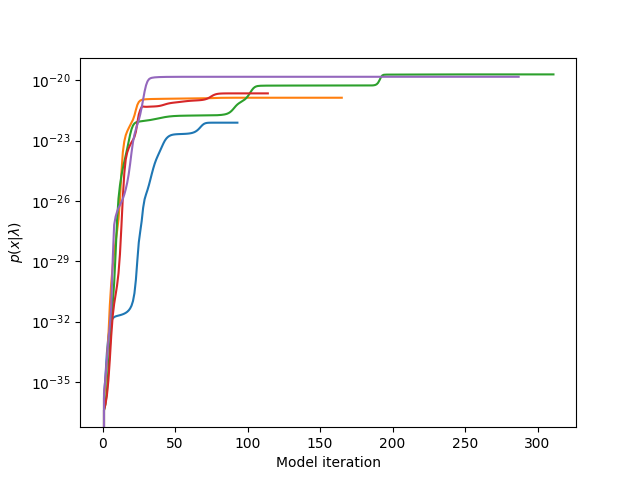
\includegraphics[width=.95\textwidth]{EM2.png}
    \caption{}
    \label{fig:em1}
    \end{center}
    \end{subfigure}%
    \begin{subfigure}{.5\textwidth}
        \begin{center}
        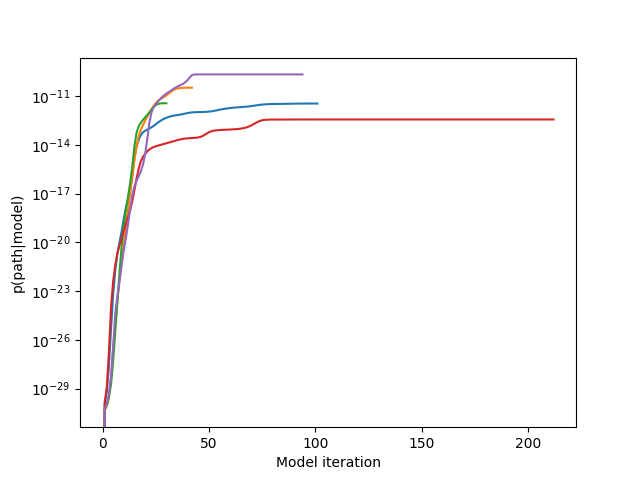
\includegraphics[width=.95\textwidth]{EM.png}
        \caption{}
        \label{fig:em2}
    \end{center}
        \end{subfigure}%
        \caption{Convergence of $p(x|\lambda)$ to local maxima for 2 values of $x$ each using 5 randomly initialised $\lambda$.}
    \label{fig:em}
    \end{center}
    \end{figure}